% mn2esample.tex
%
% v2.1 released 22nd May 2002 (G. Hutton)
%
% The mnsample.tex file has been amended to highlight
% the proper use of LaTeX2e code with the class file
% and using natbib cross-referencing. These changes
% do not reflect the original paper by A. V. Raveendran.
%
% Previous versions of this sample document were
% compatible with the LaTeX 2.09 style file mn.sty
% v1.2 released 5th September 1994 (M. Reed)
% v1.1 released 18th July 1994
% v1.0 released 28th January 1994

% \documentclass[useAMS,usenatbib,usegraphicx]{mn2e}

\documentclass[a4paper,12pt,useAMS,usenatbib,revtex4]{mn2e}
% If your system does not have the AMS fonts version 2.0 installed, then
% remove the useAMS option.
%
% useAMS allows you to obtain upright Greek characters.
% e.g. \umu, \upi etc.  See the section on "Upright Greek characters" in
% this guide for further information.
%
% If you are using AMS 2.0 fonts, bold math letters/symbols are available
% at a larger range of sizes for NFSS release 1 and 2 (using \boldmath or
% preferably \bmath).
%
% The usenatbib command allows the use of Patrick Daly's natbib.sty for
% cross-referencing.
%
% If you wish to typeset the paper in Times font (if you do not have the
% PostScript Type 1 Computer Modern fonts you will need to do this to get
% smoother fonts in a PDF file) then uncomment the next line
% \usepackage{Times}

%%%%% AUTHORS - PLACE YOUR OWN MACROS HERE %%%%%
\usepackage{lineno}
% \linenumbers
\usepackage{graphicx}
\usepackage{longtable}
\usepackage{amssymb}
\usepackage{tabularx, blindtext}
\usepackage{lscape}
\usepackage{url}
%%%%%%%%%%%%%%%%%%%%%%%%%%%%%%%%%%%%%%%%%%%%%%%%

\title[Choosing the right law for minimum bias retrieval of transit parameters from transit lightcurves]
{Limb-darkening and exoplanets II: choosing the right law for minimum bias retrieval of transit parameters from transit lightcurves}
\author[Espinoza \& Jord\'an ]{
N\'estor Espinoza$^{1,2}$\thanks{E-mail:nespino@astro.puc.cl}, 
Andr\'es Jord\'an$^{2,1}$\thanks{E-mail: ajordan@astro.puc.cl}\\ 
$^{1}$Millennium Institute of Astrophysics, Vicu\~na Mackenna 4860, Santiago, Chile\\
$^{2}$Instituto de Astrof\'isica, Pontificia Universidad Cat\'olica de Chile, Vicu\~na Mackenna 
4860, Santiago, Chile}
\begin{document}

\date{}

\pagerange{\pageref{firstpage}--\pageref{lastpage}} \pubyear{2015}

\maketitle

\label{firstpage}

\begin{abstract}
It has recently been demonstrated that the parametrization of the limb-darkening effect on a star has a direct impact 
on the parameters retrieved from transit lightcurves such as the exoplanet's radius, scaled semi-major axis and inclination. However, 
studies regarding this issue have only focused on the widely used quadratic limb-darkening law, leaving outside of the analysis 
other proposed laws that in fact are better descriptors of model intensity profiles. In this work, we show that in fact 
laws such as the logarithmic, square-root and three-parameter do a better job at retrieving the mentioned parameters from transit 
lightcurves than the widely used quadratic law and, as such, we recommend using those instead. We also detail when to use each of those, 
which we note has a dependence on both stellar and transit parameters. In addition, we demonstrate that the exponential law should not be 
used as it fundamentally non-physical, typically producing a divergence towards negative intensities at the limb.
\end{abstract}

\begin{keywords}
stellar astrophysics -- limb darkening -- exoplanets: transits.
\end{keywords}

% #################################################################################################################################
% #################################################################################################################################
% #################################################################################################################################
% ############################################# SECTION 1 #########################################################################
% #################################################################################################################################
% #################################################################################################################################
% #################################################################################################################################

\section{Introduction}
In the past decade, the study of transiting exoplanets has been evolving from discovery to very precise characterization of these systems, 
thanks to the exquisit precision allowed mainly by space-based observatories such as the Hubble Space Telescope (HST) and the Kepler mission. 
This in turn has allowed the exoplanet community to study precise mass-radius diagrams \citep[see, e.g.,][and references therein]{wm2014}, and in turn raise 
questions about the possibility of not only obtaining a precise determination of the internal composition of small, rocky exoplanets based on mass-radius
measurements \citep{dorn2015} or of their atmospheric fractions from radius measurements alone \citep{WL2015}, but also has allowed for the determination of
derived parameters of the systems that even allow for the obtention of stellar parameters directly from transit lightcurves through techniques such as asterodensity
profiling \citep{sm2003,kipping2014AP}, or of the detection of atmospheric features in exoplanet atmospheres through the technique of transmission spectroscopy. 
All these studies and techniques rely on the retrieval of precise and accurate transit parameters from transit lightcurves.

In a recent study \citep[][hereafter referred as EJ15]{ej2015}, we showed that the accuracy is actually catching up with the precision 
of these measurements due to our poor understanding of the limb-darkening effect. In particular, we showed that there are important 
biases both when fixing and fitting the limb-darkening coefficients in the light curve fitting process, with the latter arising from the fact 
that the popular and widely used quadratic law is unable to model the complex intensity profile of real stars and the former arising for this 
same reason plus the fact that different methods of fitting the model intensity profiles give rise to different limb-darkening coefficients and 
from the fact that we have an imperfect knowledge of the real intensity profiles of stars. This showed that fixing the limb-darkening coefficients is 
actually the worst option if one is willing to obtain precise \textit{and} accurate transit parameters, because the biases arise from three different sources, 
with the last one (the fact that we do not have a perfect modelling of the stellar intensity profiles of real stars) having an unknown but possibly 
large impact on them. 

Given the above, unless the data quality is really poor (and one is willing to sacrifice bias over variance), there is actually no good reason why one would 
actually want to fix the limb-darkening coefficients in the transit fitting process (assuming computational resources are not an issue). However, although fitting the 
limb-darkening coefficients seems to be a good solution to the accuracy problem, this still has the issue of the low flexibility of the quadratic limb-darkening 
law which still causes important biases on the retrieved transit parameters according to EJ15, which can be a large as $\sim 1\%$ for the planet-to-star 
radius ratio $R_p/R_*$, $\sim 2\%$ for the scaled semi-major axis, $a/R_*$, and $2\%$ for the inclination, where $R_p$ is the planetary radius, $R_*$ 
the stellar radius and $a$ the semi-major axis. The importance for missions like Kepler and for future missions like the Transiting Exoplanet Survey 
Satellite \cite[TESS,][]{ricker2014} is evident when looking at the most recent results from the Kepler mission: if we focus on the planet-to-star radius ratio 
alone, which according to EJ15 has an accuracy bias on the order of $\sim 0.2\%$, a query to the Nasa Exoplanet Archive\footnote{\url{http://exoplanetarchive.ipac.caltech.edu/}; query done on 29/09/2015.} shows that out of 3063 planetary candidates, 933 ($26\%$) have precisions better than 
$0.2\%$, and out of 1001 Kepler confirmed exoplanets, 463 (46\%) do too. This means that at least\footnote{It is important to note that this is an 
underestimate of the number of planet candidates with estimation errors, due to the fact that the Kepler pipeline makes use of fixed limb-darkening 
coefficients using the quadratic law \citep{rowe2015}, which as explained here and estimated in EJ15, gives rise to more severe biases than the one used for this 
estimation} $26\%$ of the planet candidates (from which, e.g., population studies, which rely on averaging out \textit{random} and not \textit{systematic} 
uncertainties like the ones introduced by limb-darkening) and almost half of the confirmed exoplanets (from which, e.g., characterization studies are 
based on) have important systematic errors.

An obvious solution to the above mentioned problem if one decides to fit the limb-darkening coefficients is to try to use \textit{other} laws to describe 
the intensity profile of stars. Although the non-linear law proposed by \cite{claret2000} seems to be the most flexible, the fact that it has four free parameters 
does not make it a very attractive choice in this scheme if one is willing to replace the quadratic law. However, laws with fewer parameters have been proposed, 
with the two-parameter laws being the exponential proposed by \cite{claret2003}, the logarithmic proposed by \cite{klinglesmith1970} and the square-root proposed 
by \cite{diazgimenez1992}. In addition, a very flexible three-parameter law was also proposed by \cite{sing2009}. These lower parameter laws seem to be 
very attractive for transit fitting purposes, due to their flexibility at following different intensity profiles \citep[see, e.g., ][for a comparison between the goodness of 
fit to ATLAS model atmospheres of the mentioned two-parameter laws which outperform the linear and quadratic laws in terms of following the intensity 
profiles]{howarth2011} and their low number of parameters.

Despite the attractive nature of the mentioned limb-darkening laws, testing their performance at retrieving transit parameters from transit 
lightcurves was a problem until recently for two reasons. First, there was no published algorithm that 
was capable of efficiently generating fast and accurate transit lightcurves using all of these non-standard laws. However, recently \cite{batman2015} published an 
algorithm that does exactly this called \texttt{batman}, enabling one then to generate transit lightcurves very efficiently with any arbitrary limb-darkening law. 
The second problem was that it was not clear how to sample limb-darkening coefficients in an informative (i.e., sampling all the physically possible parameter 
space) and efficient way for all of these laws. \cite{kipping2015} recently derived an algorithm to sample parameters from the three-parameter law by imposing physically plausible constrains on the intensity profiles which derived in constrains on the limb-darkening coefficients being fitted, while \cite{kipping2013}, using the same principle, derived an algorithmic way of 
doing this for two-parameter laws. However, he found that his algorithm was not applicable to the exponential law and thus no constrains for this law could 
be derived. In addition to this, the form of the logarithmic law used in \cite{kipping2013} differs from the standard one proposed by \cite{klinglesmith1970}, 
which is actually the one used in \texttt{batman}. Thus, in order to sample coefficients from this limb-darkening law, one first has to derive an efficient 
informative sampling scheme for this standard form of the law. 

In this work, we aim at testing how well do these non-standard laws perform at retrieving transit parameters from transit lightcurves, and compare them to 
the retrievals done by the standard quadratic limb-darkening law. For this, we first follow \cite{kipping2013} in order to derive an efficient sampling scheme 
for the standard form of the logarithmic and exponential laws, and show that the latter is actually \textit{always} non-physical in the sense proposed by 
\cite{kipping2013}. Then, we simulate transit lightcurves and perform a simulation study similar to the one done in EJ15 using the derived sampling schemes 
for the logarithmic law and the ones detailed in \cite{kipping2013} for the other two-parameter laws and \cite{kipping2015} for the three-parameter law, 
detailing when one law should be preferred over the other. 

This work is organised as follows. In \S2, we first revisit the logarithmic and exponential 
laws in order to try to derive an efficient informative sampling strategy following the methods in \cite{kipping2013} for the standard forms of these laws. 
In \S3 we use those results in addition to the ones published by \cite{kipping2013} and \cite{kipping2015} in order to simulate transit lightcurves to test 
how well these laws perform in retrieving transit parameters. In \S4 we present a discussion and conclusions of our work.

% #################################################################################################################################
% #################################################################################################################################
% #################################################################################################################################
% ############################################# SECTION 2 #########################################################################
% #################################################################################################################################
% #################################################################################################################################
% #################################################################################################################################

\section{Efficient sampling of coefficients from the logarithmic and exponential laws revisited}

As explained in the introduction, an informative and efficient sampling of limb-darkening coefficients 
in order to fit them to transit lightcurves is fundamental. Motivated by this, \cite{kipping2013} introduced 
an algorithm which first imposes physically plausible constrains on the intensity profiles, namely, an everywhere 
positive intensity profile ($I(\mu)>0$) and a decreasing intensity profile from center to limb ($\partial I(\mu)/\partial \mu>0$), 
which in turn impose constrains on the parameters of the studied two-parameter law. With these constrains at hand, 
\cite{kipping2013} devised a triangular sampling strategy which only require sampling two uniformly distributed numbers between 
0 and 1, $q_1$ and $q_2$, which through a transformation can be converted in order to sample coefficients that follow the 
derived constrains. This was done in that work for the most popular two-parameter limb-darkening laws with the exception of the 
exponential limb-darkening law, whose derived constrains on the coefficients were not enough 
to use the triangular sampling technique, and for the typical form of the logarithmic law, which is 
different to the one used in \cite{kipping2013}. 

We here first derive an informative and efficient sampling strategy for the typical form of the logarithmic law and then 
we study the exponential law, for which we conclude that deriving an efficient sampling strategy is actually 
\textit{impossible}; this implies that the law is fundamentally non-physical and, therefore, should not be used. 

\subsection{Efficient sampling from the logarithmic law}
As described in \cite{klinglesmith1970}, the logarithmic law is given by
\begin{eqnarray}
\label{loglaw} I(\mu) = 1 - l_1(1-\mu)-l_2\mu \ln\mu.
\end{eqnarray}
However, \cite{kipping2013} derived the constrains for a law similar (but 
not the same) to the original logarithmic law, given by
\begin{eqnarray*}
I_K(\mu) = 1 - A(1-\mu)-B\mu (1-\ln\mu),
\end{eqnarray*}
which can be viewed as the original logarithmic law with an extra linear term. Given that this 
is not the original law many authors have adopted both to obtain limb-darkening coefficients 
and to model transit lightcurves, we here derive a sampling strategy for the original logarithmic 
limb-darkening law given in eq. (\ref{loglaw}). To do this, we start by imposing 
physically plausible constrains on the intensity profiles. The constrain of an everywhere positive intensity profile implies
\begin{eqnarray*}
 l_1(1-\mu)+l_2\mu \ln\mu < 1 �&\forall& 0<\mu<1.
\end{eqnarray*}
In order to ensure this condition, we need to find the extrema of the expression in the 
left-hand side. We note that the maximum of the expression is obtained only if $l_2<0$, 
while the minimum of the expression is obtained if $l_2>0$. In both cases, this happens 
at $\mu_e=\exp [(l_1-l_2)/l_2]$, where we have assumed $l_2 \neq 0$. If $l_2=0$, then 
we obtain the inequality $l_1(1-\mu)<1$, which implies $l_1<1$, constraint we will see 
is valid for all the possible values of $l_2$. In the case $l_2>0$, because 
$\mu_e$ gives a minimum, 
$\mu\to 1$ and $\mu \to 0+$ maximise the expression in the desired range. The first limit 
gives the trivial constrain $1>0$, while the second limit gives the constrain $l_1<1$. In 
the case $l_2<0$, replacing $\mu_e$ in the expression leads to the constrain
\begin{eqnarray*}
\frac{l_1-1}{\mu_e} < l_2,
\end{eqnarray*}  
which, because $l_2<0$, again implies $l_1<1$. The condition 
for a decreasing intensity profile from center to limb, on the other hand, leads to the 
condition
\begin{eqnarray*}
l_1-l_2(1+\ln\mu) > 0 �&\forall& 0<\mu<1.
\end{eqnarray*}
The left-hand side has, again, a division depending on the sign of $l_2$. If $l_2>0$, then 
the expression is convex and has no absolute minimum. It can be seen that then the 
expression is always satisfied for $0<\mu < 1$. In the limit $\mu \to 1$, the expression leads 
to the condition $l_1>l_2$. For the $\mu \to 0^+$ limit, however, no condition can be derived 
because the expression diverges. If $l_2<0$, on the other hand, the expression is concave, and 
it does not have an absolute maximum. It can be seen, however, that the expression in the limit 
$\mu \to 1$, leads to $l_1>l_2$ just as in the first case, but in this case the expression is not valid 
for $\mu \to 0^+$, because it goes to $-\infty$. This implies that for $l_2<0$ the inequality will 
never be satisfied in the desired range and, thus, we need $l_2>0$ in order for the profile to be 
everywhere decreasing. In summary, the derived condition for an everywhere positive intensity profile is
\begin{eqnarray*}
l_1<1,
\end{eqnarray*}
while the conditions for an everywhere decreasing intensity profile from center to limb are
\begin{eqnarray*}
l_2>0,\\
l_1>l_2.
\end{eqnarray*}

\begin{figure}
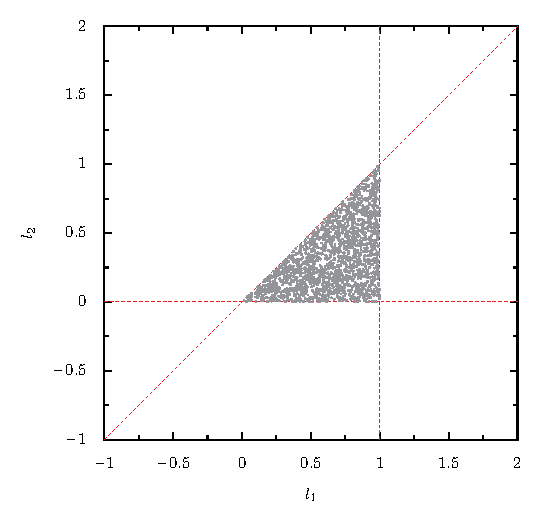
\includegraphics{sampling_simulation_log/triangular_sampling.eps}
\caption{Samples of the logarithmic limb-darkening coefficients that satisfy the derived constrains in 
this section out of $10^6$ uniformly sampled points between $-1<l_1<2$ and $-1<l_2<2$. Only 
$\sim 5\%$ of those samples satisfy such relations, shown here with red dashed lines.}
\label{triangular_sampling}
\end{figure}

Figure \ref{triangular_sampling} show these constrains geometrically. For illustration, $10^6$ points were uniformly sampled 
between $-1<l_1<2$ and $-1<l_2<2$ and a sample of those that satisfy these constrains were plotted. Only $5\%$ of them 
did satisfy such relations which demonstrates, as \cite{kipping2013} showed, the inefficiency of using such sampling strategy 
to draw physically plausible limb-darkening coefficients. This is the reason why we need to use the triangular sampling technique 
described in \cite{kipping2013}.

In order to use the triangular sampling technique, one needs to re-parametrize 
the constrains in order for them to be sampled on a right-angled triangle with this angle posed in the origin. A 
parametrisation that does this is the one with
\begin{eqnarray}
\label{v1}&v_1& = 1-l_1,\\
\label{v2}&v_2& = l_2.
\end{eqnarray}
If we now consider the transformations \citep[see][]{kipping2013}
\begin{eqnarray}
\label{v1q} &v_1& = \sqrt{q_1}q_2,\\
\label{v2q} &v_2& = 1 - \sqrt{q_1},
\end{eqnarray}
sampling $q_1$ and $q_2$ from uniform distributions between $(0,1)$ leads to a sampling with the desired constrains 
between $l_1$ and $l_2$. Replacing the expressions in eqs. (\ref{v1q}) and (\ref{v2q}) in eqs. (\ref{v1}) and (\ref{v2}) gives 
\begin{eqnarray*}
l_1 &=& 1-\sqrt{q_1}q_2\\
l_2 &=& 1-\sqrt{q_1}
\end{eqnarray*}
which leads to the inverse equations
\begin{eqnarray*}
q_1 &=& (1-l_2)^2,\\
q_2 &=& \frac{1-l_1}{1-l_2}.
\end{eqnarray*}
We note that, as expected, these relations return limb-darkening coefficients that are physically plausible for this law (i.e., they follow 
the derived constrains). Furthermore, we note these relations are different to the ones derived in \cite{kipping2013}; these are only applicable 
for his form of the logarithmic law.

\subsection{The exponential law is non-physical}
We now study the exponential limb-darkening law. This law was introduced by \cite{claret2003}, and is given by
\begin{eqnarray*}
I(\mu) &=& 1-e_1(1-\mu)-e_2/(1-e^\mu).
\end{eqnarray*}
\cite{kipping2013} tried to apply the same methods used for the other two-parameter laws in order to 
derive constrains and hence an efficient sampling scheme for the coefficients of this law, but observed that the triangular 
sampling technique was not applicable in this case because the imposed physical constrains were not 
able to yield a sufficient number of relations between the coefficients for it to 
be used. However, apparently overlooked by \cite{kipping2013} is the fact that the exponential law will \textit{never} 
yield physically plausible coefficients for $0<\mu<1$, because the conditions of an everywhere positive and decreasing 
intensity profile from center to limb cannot be satisfied at the same time, as we now show.

We start by imposing an everywhere positive intensity profile for this law. This leads to the relation
\begin{eqnarray*}
e_1(1-\mu)+e_2/(1-e^\mu)<1 &\forall& 0<\mu<1,
\end{eqnarray*}
and the objective is to study the left-hand side. We note that this expression has a minimum if 
$e_2<0$, while it has a maximum when $e_2>0$. We see that in the first case, as $\mu \to 0^+$, 
the expression tends to $\infty$, and therefore the expression is never satisfied; this implies that 
$e_2$ cannot be less than zero in order to have an everywhere positive intensity profile. On the 
other hand, if we impose an everywhere decreasing intensity profile for this law from center to 
limb, one can note this leads to the constrain:
\begin{eqnarray*}
e_1 - e_2 \frac{e^\mu}{(1-e^\mu)^2}>0 &\forall& 0<\mu<1.
\end{eqnarray*}
The form of the left-hand side expression again depends on the value of $e_2$ in the same way 
as before; however, in this case there is no absolute maximum or minimum and, thus, it suffices 
to study the expression at the borders. We note that in order for the expression to be satisfied 
for all the values of $\mu$, $e_2<0$, because only in this case the expression goes to $\infty$ 
when $\mu \to 0^+$. Because in order for the exponential law to have an everywhere positive intensity 
profile this condition was ruled out, this implies that both conditions cannot be met at the 
same time and, thus, there is no combination of coefficients $(e_1,e_2)$ that satisfy the physically 
plausible conditions suggested by \cite{kipping2013} for this law: in this sense, the exponential 
law introduced by \cite{claret2003} is non-physical.

\begin{figure}
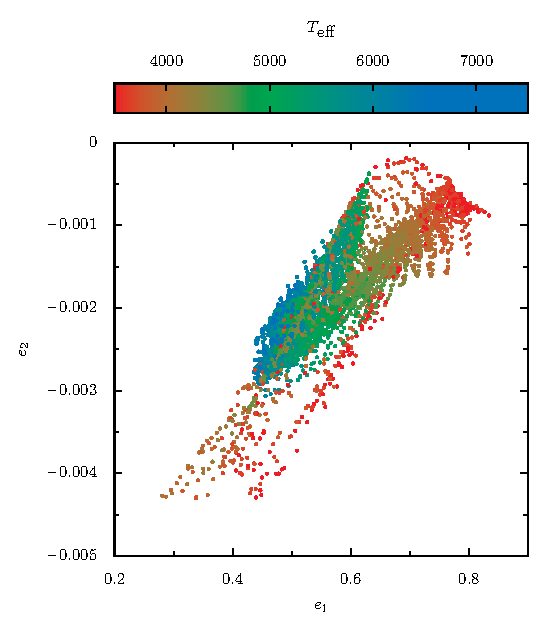
\includegraphics{coefficients_check_exp/exponential_ldcs.eps}
\caption{Limb-darkening coefficients for the exponential law obtained using the methods described in 
EJ15 with the Kepler bandpass for all the stars in the ATLAS models with $T_\textnormal{eff}<9000$ K. As 
can be seen, $e_2<0$, which implies that all the fitted intensity profiles are not everywhere positive and, 
thus, non-physical.}
\label{exponential_ldcs}
\end{figure}

We note that typical values obtained by fitting the exponential law to model atmospheres give $e_2<0$, which means that 
most of the profiles fitted to model atmospheres do not have an everywhere positive intensity profile. To illustrate 
this, in Figure \ref{exponential_ldcs} we plot all the coefficients fitted using the exponential law following the methods 
of EJ15 using the Kepler bandpass for stars of interest for exoplanet studies ($T_\textnormal{eff}<9000$ K) obtained with 
the ATLAS models. In order to 
see at which value of $\mu$ the profile starts to be negative, we note that this happens as $\mu \to 0^+$. Here 
$1/(1-e^\mu) \approx -1/\mu$, which gives
\begin{eqnarray*}
I(\mu) &\approx& 1-e_1(1-\mu)+e_2/\mu.
\end{eqnarray*}
The intensity profile then, touches $I(\mu)=0$ around
\begin{eqnarray*}
\mu_0 \approx \frac{e_1-1 \pm \sqrt{(1-e_1)^2 - 4e_1e_2}}{2e_1}
\end{eqnarray*}
According to Figure \ref{exponential_ldcs}, $e_1\sim 0.6$, while $e_2 \sim - 2\times 10^{-3}$, which gives $\mu_0 \sim 0.005$, 
so the law starts giving negative values very close to (but not at) the limb, as we predicted. We note that typical transit observations are capable 
of sampling these points by chance, with high cadence observations as the ones done by the Kepler mission and the ones that will 
be done with the future TESS mission \citep{ricker2014} having an almost certain chance of sampling points inside those ranges. 
Furthermore, as the generation of transit lightcurves for laws like the exponential requiere either numerical integration or the usage 
of clever approximations that usually sample more points close to the limb \citep[which is the case for e.g., the \texttt{batman} code,][]{batman2015}, this law is doomed to produce numerical errors in transit lightcurves due to this fact. Because of these reasons, it is advisable not to use this law in real 
applications.

% #################################################################################################################################
% #################################################################################################################################
% #################################################################################################################################
% ############################################# SECTION 3 #########################################################################
% #################################################################################################################################
% #################################################################################################################################
% #################################################################################################################################

    
\section{Biases in transit parameters using two-parameter laws}
Having solved the issues regarding the sampling of limb-darkening coefficients from the 
logarithmic and exponential laws, we now turn to the study of the 
biases introduced on retrieved transit parameters in the transit fitting process introduced by using different limb-darkening laws. In 
order to perform this study, we perform a similar study as the one done in EJ15, but now 
(1) using the \texttt{batman} transit code described in \cite{batman2015}, (2) using three different two-parameter 
laws: the quadratic, logarithmic and square-root laws (with the exponential law left out of our analysis because, 
as was shown in \S 2.2, it's fundamentally non-physical) and the three-parameter law and (3) smaller steps in 
the planet-to-star radius ratio, $p=R_p/R_*$, in order to illustrate the evolution of the biases with this parameter 
in a cleaner way: small ratios ($p=0.01$), medium ratios ($p=0.07$) and large ones ($p=0.13$) . 

As in EJ15, we simulate transit lightcurves for planets orbiting around host stars with solar metallicity, 
gravity and microturbulent velocity between 3500 K and 9000 K, with the mentioned planet-to-star radius ratios, 
values of the scaled semi-major axis of $a_R = a/R_* = \{3.27, 3.92, 4.87, 6.45, 9.52, 18.18, 200\}$ and different 
impact parameters. The transits are simulated using a non-linear law in order to emulate "real" intensity profiles, 
with the coefficients generated using the ATLAS models and the same methods as the ones used in EJ15 with the 
Kepler bandpass. The transits were then fitted using free limb-darkening coefficients with the mentioned laws.

For the simulations, the applied strategies in this work to sample physically plausible coefficients from two-parameter laws 
are as follows, all of which use numbers $q_1 \in (0,1)$ and $q_2 \in (0,1)$:
\begin{itemize}
\item For the quadratic limb-darkening law, we fit for the numbers $q_1 = (u_1 + u_2)^2$ and $q_2 = u_1/2(u_1+u_2)$. 
To obtain the coefficients from those fitted numbers, we use the relations $u_1 = 2\sqrt{q_1}q_2$ and $u_2 =\sqrt{q_1}(1-2q_2)$, 
which are derived in \cite{kipping2013}.
\item For the square-root law, we fit for the numbers $q_1 = (s_1 + s_2)^2$ and $q_2 = s_2/2(s_1+s_2)$. 
To obtain the coefficients from those fitted numbers, we use the relations $s_1 = \sqrt{q_1}(1-2q_2)$ and $s_2 =2\sqrt{q_1}q_2$, 
which are derived in \cite{kipping2013}.
\item For the logarithmic law, we fit for the numbers $q_1 = (1-l_2)^2$ and $q_2 = (1-l_1)/(1-l_2)$. 
To obtain the coefficients from those fitted numbers, we use the relations $l_1 = 1-\sqrt{q_1}q_2$ and $l_2=1-\sqrt{q_1}$, 
which are derived in \S 2.1.
\end{itemize}
For the three-parameter law, we use the formalism and codes described in \cite{kipping2015}. As explained before, analyses for the 
exponential law were not made as it is fundamentally non-physical. The code used to generate these simulations has been published 
in GitHub\footnote{\url{http://www.github.com/nespinoza/ld-simulations/}}, and can be used to perform analyses in a finer grid to the ones 
published here. 
\subsection{The case of central transits}
\begin{figure*}
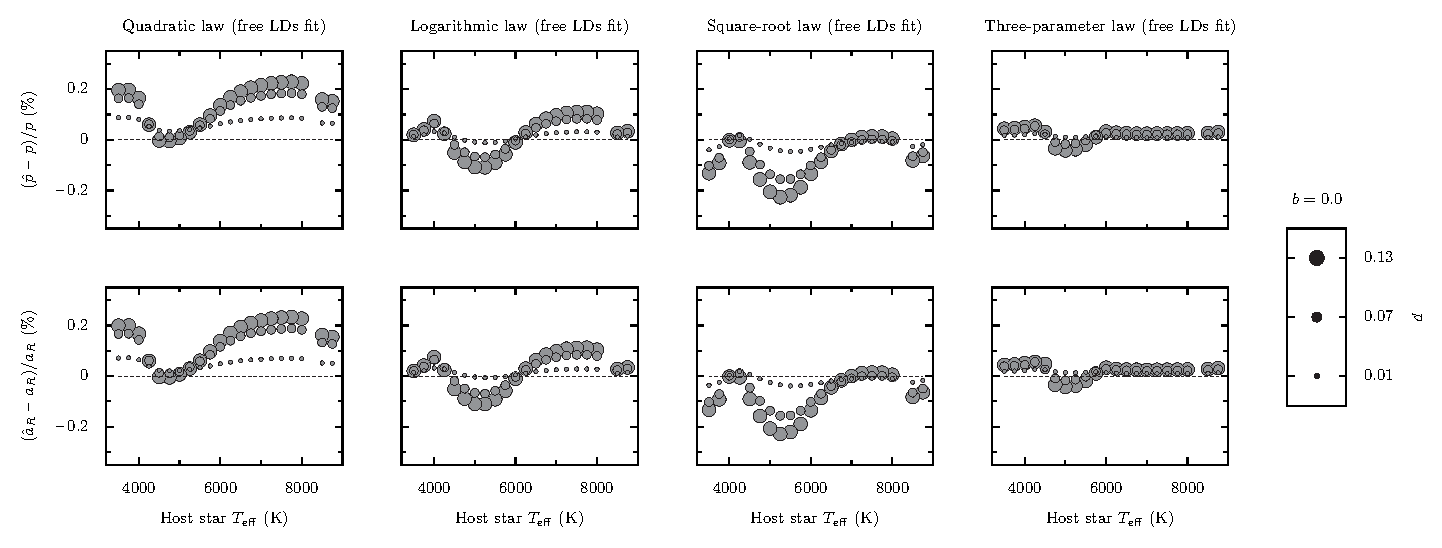
\includegraphics[scale=0.8]{bias_transit_params/all_laws/b_0.0/simulation_b_00_float.eps}
\caption{Results of fitting transit lightcurves as described in \S 3.1 with the limb-darkening coefficients as free parameters. We only 
plot the size of the points which represent the input values of $p$.}
\label{central_sims}
\end{figure*}

The results of the simulations for central transits (i.e., $b=0$) are shown in Figure \ref{central_sims}, with the sizes of the points representing the 
input values of $p$. The upper panels showing the biases 
introduced on the planet-to-star radius ratio, $p$, and the lower panels showing the biases introduced on the scaled semi-major axes, $a_R$. From left to right, 
the panels show the biases introduced by using a quadratic law, a logarithmic law, a square-root law and a three-parameter law in the transit fitting 
procedures leaving the corresponding limb-darkening coefficients as free parameters. The dependence with the input values of $a_R$ are 
not shown as the bias seem to be almost independent of this parameter in this case (this can be also seen by looking at the lower panels of Figure 10 in EJ15, which 
give the same results as the ones shown here for the quadratic law, showing a nice agreement between the simulations done with our implementation of 
the \cite{ma2002} codes for the transit light curve generation and the \texttt{batman} code). 

As can be seen from the figure, different limb-darkening laws have different behaviours in retrieving $p$ and $a_R$, with a dependence on the input value of 
$p$, and also depending on the temperature of its host star. First, it is interesting to note that the logarithmic law does a very good job at retrieving 
the parameters of small planet-to-star radius ratios, even at the level of the three-parameter law for stars with $T_\textnormal{eff}<6000$ K, and also for medium 
and large planet-to-star radius ratios with host-stars with $T_\textnormal{eff}<4000$ K (which makes this law perfect for present and future transit 
detection and characterisation around M-dwarfs). The quadratic law, on the other hand, is only the best among the options for host-stars between 
$4250<T_\textnormal{eff}<5500$ K, with the logarithmic law being the best in the $5500<T_\textnormal{eff}<6250$ K range, and the square-root law 
being the best for planets around host stars with temperatures between $6250<T_\textnormal{eff}<8000$ K. Hotter than this, the best option in terms 
of accuracy is the three-parameter law.

It is interesting to emphasise that although the biases introduced by the quadratic law might seem to be small, as mentioned in the introduction and in 
EJ15 they are significant for several candidate and confirmed exoplanets. However, choosing the right law in this case can help to achieve the same 
level of accuracy than the level of precision that Kepler achieves for most planets. In this case, for example, accuracies on the order of $\sim 0.01\%$ can 
be achieved for $p$ with a careful selection of a two-parameter law, and exoplanets with precisions better than that according to a query to the Nasa Exoplanet 
Archive\footnote{Query done on 29/09/2015.} form only $0.58\%$ of all candidate exoplanets and $1.2\%$ of the confirmed exoplanets. For the remaining 
exoplanets requiring a better accuracy, a new law might have to be created, as this precision is also the limit of the three-parameter law (which has a precision 
on $p$ around $\sim 0.01\%$ for stars with temperatures larger than $T_\textnormal{eff}=6000$ K). Studying new limb-darkening laws, however, 
is out of the scope of the present work.

\subsection{The case of non-central transits}
\begin{figure*}
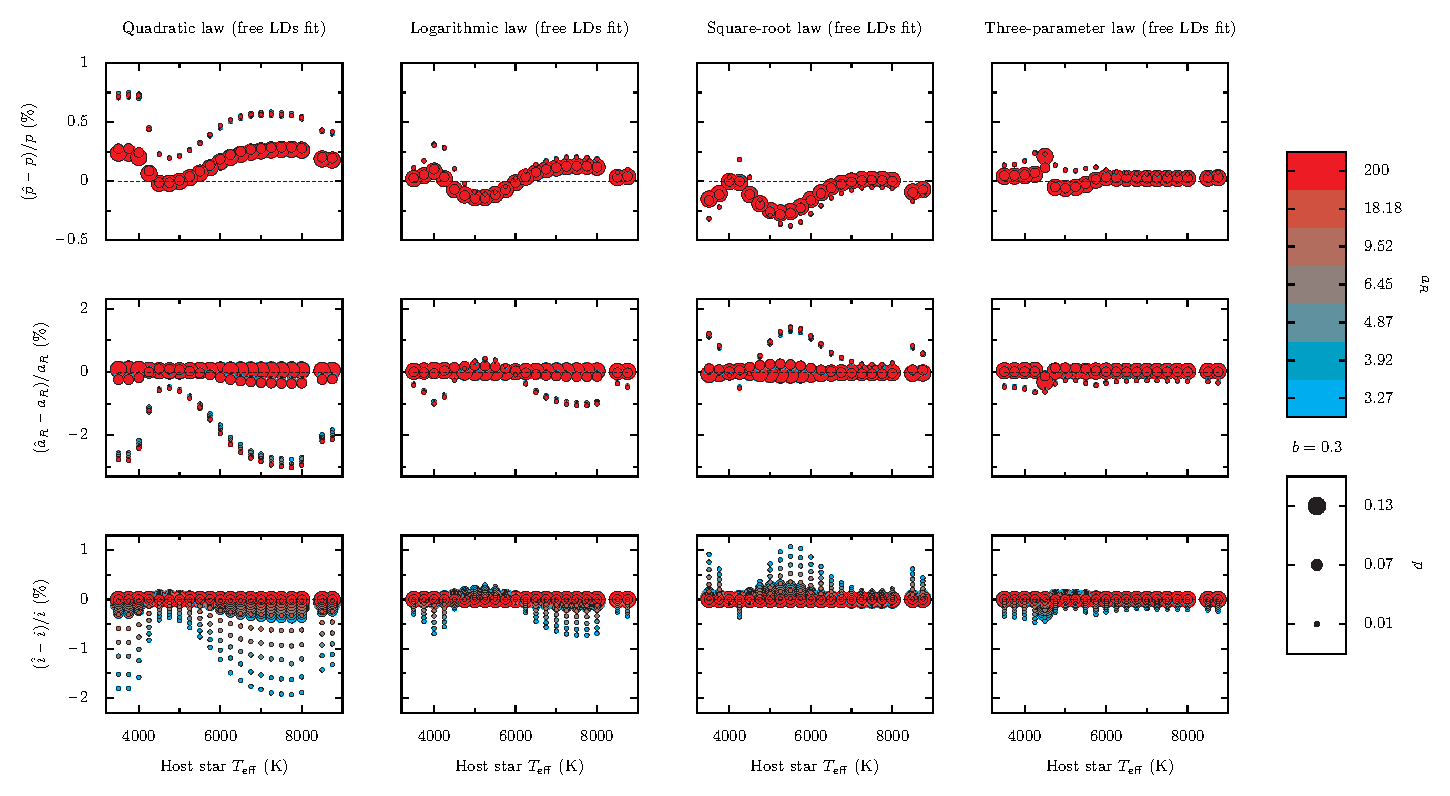
\includegraphics[scale=0.8]{bias_transit_params/all_laws/b_0.3/simulation_b_03_float.eps}
\caption{Results of fitting transit lightcurves as described in \S 3.1 with the limb-darkening coefficients as free parameters, but for low impact 
parameter transits ($b=0.3$). The size of the points represent the input values of $p$, while their color represent the input values of $a_R$.}
\label{small_b_sims}
\end{figure*}

\begin{figure*}
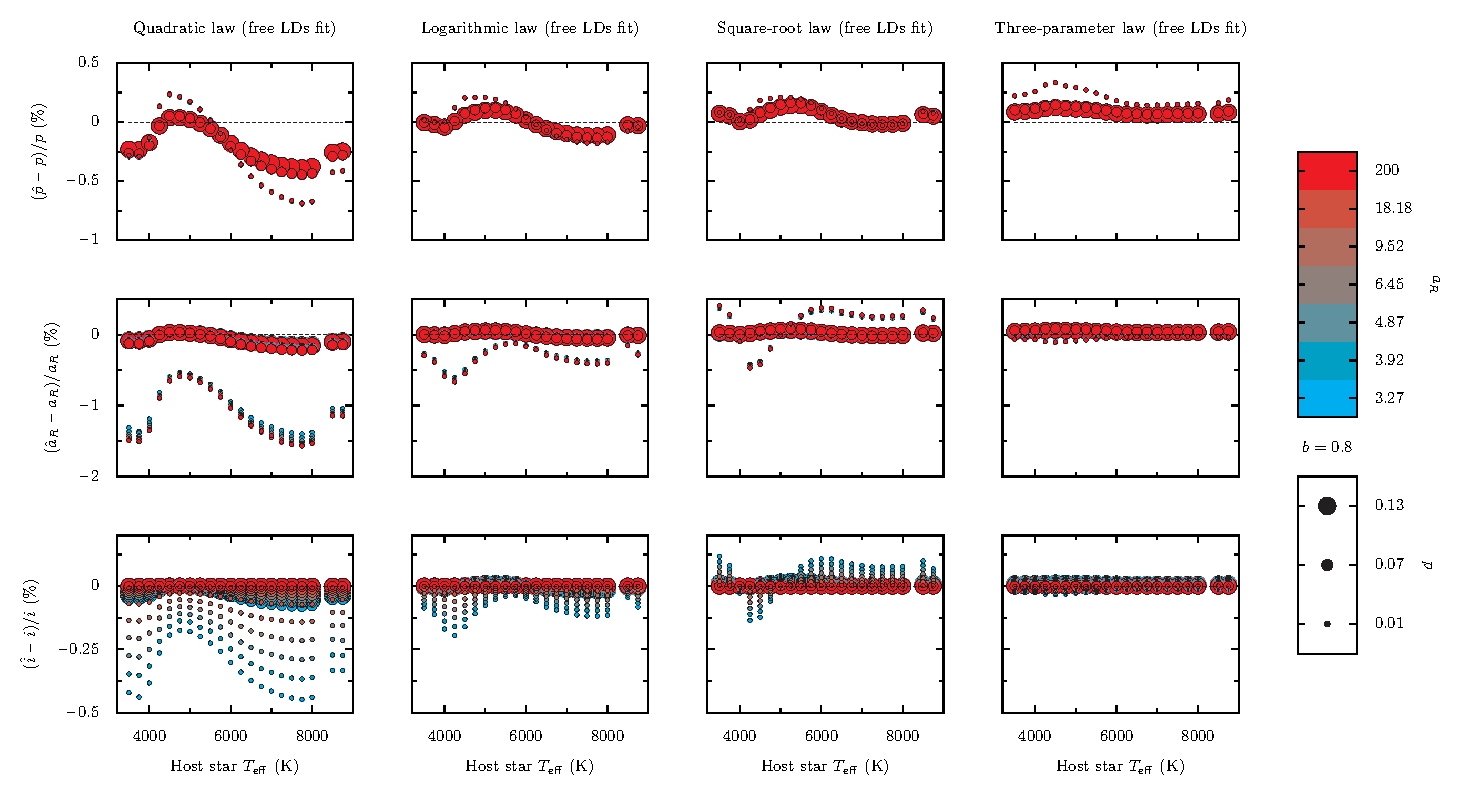
\includegraphics[scale=0.8]{bias_transit_params/all_laws/b_0.8/simulation_b_08_float.eps}
\caption{Results of fitting transit lightcurves as described in \S 3.1 with the limb-darkening coefficients as free parameters, but for high impact 
parameter transits ($b=0.8$). The size of the points represent the input values of $p$, while their color represent the input values of $a_R$.}
\label{big_b_sims}
\end{figure*}

Figures \ref{small_b_sims} and \ref{big_b_sims} show the results for low ($b=0.3$) and high ($b=0.8$) input impact parameters respectively. In these cases, 
we see that the biases are in general worse for smaller values of $p$ and $a_R$, i.e., for a given stellar radius, for smaller, close-in planets. We can 
also see that, again, a careful selection of the law to be used can allow one to minimize the biases on the retrieved transit parameters. For example, if 
the objective were to obtain $p$ with minimum bias for a low impact-parameter transit, then for host stars colder than $4000$ K the best option is to use 
either the logarithmic or the three-parameter law, which show biases on the order of $\sim 0.1\%$. In contrast, using the quadratic law for transits around 
those host stars the biases introduced on this parameter are on the order of $\sim 0.75\%$, i.e., almost an order of magnitude improvement in the accuracy. 

Overall, as expected, the law that retrieves the parameters with minimum bias in low impact-parameter transits is the three-parameter law. However, for 
high impact-parameter transits of small planets, the logarithmic and square-root law seem to outperform this law in general if the objective is to retrieve 
a minimum bias estimator for $p$. This is due to the fact that the law is so flexible that it allows for small distortions of the transit lightcurve that, 
in this case, mimics variations that were actually attributable to $p$, adding a small but important bias on the retrieved parameter. However, for the other 
parameters ($a_R$ and $i$) this law seems to be the best choice in terms of the achieved accuracy.

\section{Discussion \& Conclusions}
In this work we have explored the different biases on the retrieved transit parameters by the usage of different limb-darkening laws. In particular, we 
explored the biases introduced by using three two-parameter laws (the quadratic, logarithmic and square-root laws) and the three-parameter law, for which 
we showed that a careful selection of the limb-darkening law to be used in a given dataset can allow one to retrieve minimum bias estimators for the transit 
parameters from transit lightcurves. In general, as shown in \S3, these two-parameter laws have ranges in which they perform at the same level or even better 
than the three-parameter law and, because of this, we encourage their use. We also discourage the usage of the exponential law which, as shown in \S2.2 is 
unphysical, and can lead to numerical errors if used on real data where sampling of points close to the limb (where the law diverges) is not uncommon.

The question of \textit{when} to use each of those laws is an important one. In particular, we have explored the relation between the \textit{real}, underlying 
transit parameters, the stellar host properties and the bias on the retrieved transit parameters, but we have stated no specific rule regarding when to use each 
law, but only guidelines based on our simulations. This was made on purpose, as the selection of which law to use has to be done in a case-by-case basis, reason 
by which we provide a code with which one can obtain the results for the same simulations for specific 
cases and with different resolutions\footnote{\url{http://www.github.com/nespinoza/ld-simulations/}}. It is important to note that in this work we have used the 
Kepler bandpass to study the relation between the biases on the retrieved transit parameters and the stellar host properties, but different bandpasses should give 
rise to slightly different functional relations because they give rise to different model intensity profiles, which are used in those simulations to approximate the 
expected intensity profile and the adequacy of each limb-darkening law at following it. As such, limb-darkening coefficients have to be calculated for each 
particular case, which is straightforward to do using the algorithms described in EJ15\footnote{\url{http://www.github.com/nespinoza/limb-darkening/}}.

\section{Acknowledgmenets}

N.E. is supported by CONICYT-PCHA/Doctorado Nacional. A.J. acknowledges 
support from FONDECYT project 1130857, the Ministry
for the Economy, Development, and Tourism Programa Iniciativa
Cient\'ifica Milenio through grant IC 120009, awarded to the
Millennium Institute of Astrophysics (MAS), and from BASAL CATA
PFB-06. 

\begin{thebibliography}{99}
\bibitem[\protect\citeauthoryear{Claret}{2000}]{claret2000} Claret, A., 2000, A\&A, 363, 1081.
\bibitem[\protect\citeauthoryear{Claret \& Hauschildt}{2003}]{claret2003} Claret, A. \& Hauschildt, P. H., 2003, 
A\&A, 412, 241.
\bibitem[\protect\citeauthoryear{D\'iaz-Cordov\'ez \& Gim\'enez}{1992}]{diazgimenez1992} D\'iaz-Cordov\'ez, J.,
\& Gim\'enez, A., 1992, A\&A, 259, 227.
\bibitem[\protect\citeauthoryear{Dorn et al.}{2015}]{dorn2015} Dorn, C., Khan, A., Heng, K., Alibert, Y., Connolly, J.,
Benz, W. \& Tackley, P., 2015, A\&A, 577, 83.
\bibitem[\protect\citeauthoryear{Kipping}{2013}]{kipping2013} Kipping, D. M., 2013, MNRAS, 435, 2152.
\bibitem[\protect\citeauthoryear{Kipping}{2014}]{kipping2014AP} Kipping, D. M., 2014, MNRAS, 440, 2164.
\bibitem[\protect\citeauthoryear{Kipping}{2015}]{kipping2015} Kipping, D. M., 2015, arXiv:1509.03483.
\bibitem[\protect\citeauthoryear{Klinglesmith \& Sobieski}{1970}]{klinglesmith1970} Klinglesmith, D. A. \&
Sobieski, S., 1970, AJ, 75, 175.
\bibitem[\protect\citeauthoryear{Espinoza \& Jord\'an}{2015}]{ej2015} Espinoza, N. \& Jord\'an, A., 2015, 
MNRAS, 450, 1879.
\bibitem[\protect\citeauthoryear{Howarth}{2011}]{howarth2011} Howarth, I., 2011, 
MNRAS, 413, 1515.
%\bibitem[\protect\citeauthoryear{Hebb et al.}{2009}]{Hebb2009} Hebb et al., 2009, ApJ, 693, 1920.
%\bibitem[\protect\citeauthoryear{Kreidberg et al.}{2013}]{Kreidberg2013} Kreidberg et al., 2013, Nature, 505, 69.
\bibitem[\protect\citeauthoryear{Klinglesmith \& Sobieski}{1970}]{klinglesmith1970} Klinglesmith, D. A. \&
Sobieski, S., 1970, AJ, 75, 175.
\bibitem[\protect\citeauthoryear{Kreidberg}{2015}]{batman2015} Kreidberg, L., 2015, arXiv:1507.08285.
\bibitem[\protect\citeauthoryear{Mandel \& Agol}{2002}]{ma2002} Mandel, K \& Agol, E., 2002, ApJ,
580, L171.
%\bibitem[\protect\citeauthoryear{Mandell et al.}{2013}]{Mandell2013} Mandell et al., 2013, ApJ, 779, 128.
\bibitem[\protect\citeauthoryear{Ricker et al.}{2014}]{ricker2014} Ricker et al., 2014, SPIE, 9143.
\bibitem[\protect\citeauthoryear{Rowe et al.}{2015}]{rowe2015} Rowe et al., 2015, ApJS, 217, 16.

\bibitem[\protect\citeauthoryear{Seager \& Mall\'en-Ornelas}{2003}]{sm2003} Seager, S. \& Mall\'en-Ornelas, G., 2003, ApJ, 585, 1038.
\bibitem[\protect\citeauthoryear{Sing et al.}{2009}]{sing2009} Sing, D. K., D\'esert, J.-M.,
Lecavelier Des Etangs, A., Ballester, G. E., Vidal-Madjar, A., Parmentier, V., Hebrard, G. \& Henry, G. W.,
2009, A\&A, 505, 891.
%\bibitem[\protect\citeauthoryear{Sing et al.}{2013}]{Sing2013} Sing et al., 2013, MNRAS, 436, 2956.
%\bibitem[\protect\citeauthoryear{Stevenson et al.}{2014}]{Stevenson2014} Stevenson et al., 2014, AJ, 147, 161.
%\bibitem[\protect\citeauthoryear{Swain et al.}{2013}]{Swain2013} Swain et al., 2013, Icarus, 225, 432.
\bibitem[\protect\citeauthoryear{Weiss \& Marcy}{2014}]{wm2014} Weiss, L. \& Marcy, G., 2014, ApJ, 783L, 6.
\bibitem[\protect\citeauthoryear{Wolfgang \& Lopez}{2015}]{WL2015} Wolfgang, A. \& Lopez, E., 2015, ApJ, 806, 183.
\end{thebibliography}

%\appendix


%if $e_2<0$, then the profile diverges to $-\infty$ as $\mu\to 0$ (because the term $1-e^\mu$ 
%tends to 0 from the left) thus not being able to fulfil the constrain of an everywhere positive intensity profile, while for 
%$e_2>0$ the profile is strictly \textit{increasing} from center to limb, thus not being able to fulfil the constrain of an 
%everywhere decreasing intensity profile from center to limb. 



\bsp

\label{lastpage}

\end{document}
